\documentclass[10pt]{article}\usepackage[]{graphicx}\usepackage[]{color}
%% maxwidth is the original width if it is less than linewidth
%% otherwise use linewidth (to make sure the graphics do not exceed the margin)
\makeatletter
\def\maxwidth{ %
  \ifdim\Gin@nat@width>\linewidth
    \linewidth
  \else
    \Gin@nat@width
  \fi
}
\makeatother

\usepackage{Sweavel}


\usepackage{hyperref}
\usepackage{url}
\usepackage[a4paper]{geometry}
\usepackage{a4wide}
\usepackage{float}
\usepackage[english]{babel}
\usepackage[utf8]{inputenc}
\usepackage{csquotes}
\usepackage{amsmath}
\usepackage{amssymb}
\usepackage{xspace}
\usepackage[numbers]{natbib}
\bibliographystyle{unsrtnat}
\usepackage{subcaption}
\usepackage[font={small}]{caption}
\usepackage{booktabs}
\usepackage{listings}
\usepackage{cleveref}
\usepackage{lipsum}
\newcommand{\approxtext}[1]{\ensuremath{\stackrel{\text{#1}}{=}}}
\newcommand{\matr}[1]{\mathbf{#1}}
\newcommand{\partt}[2]{\ensuremath{\dfrac{\partial {#1}}{\partial {#2}}}}
\renewcommand{\d}[1]{\ensuremath{\operatorname{d}\!{#1}}} % non-italized differentials
\newcommand{\h}[0]{\ensuremath{\hbar}} % hbar
\def\changemargin#1#2{\list{}{\rightmargin#2\leftmargin#1}\item[]}
\let\endchangemargin=\endlist 
\usepackage{amsthm}
\theoremstyle{plain}
\renewcommand{\theequation}{\thesection.\arabic{equation}}
\def\changemargin#1#2{\list{}{\rightmargin#2\leftmargin#1}\item[]}
\let\endchangemargin=\endlist    
\usepackage{xcolor}
\definecolor{Red}{rgb}{0.7,0,0}
\definecolor{Blue}{rgb}{0,0,0.8}
\usepackage{verbatim}
\def\changemargin#1#2{\list{}{\rightmargin#2\leftmargin#1}\item[]}
\let\endchangemargin=\endlist
\addtolength{\oddsidemargin}{-.35in}
\addtolength{\evensidemargin}{-.35in}
\addtolength{\textwidth}{.7in}
\usepackage{multicol}

% Stephen's stuff
\newcommand{\R}{\texttt{R}}
\newcommand{\Rfunction}[1]{{\texttt{#1}}}
\newcommand{\Robject}[1]{{\texttt{#1}}}
\newcommand{\Rpackage}[1]{{\mbox{\normalfont\textsf{#1}}}}
\usepackage{xcolor}
\definecolor{Red}{rgb}{0.7,0,0}
\definecolor{Blue}{rgb}{0,0,0.8}
\hypersetup{%
pdfusetitle,
bookmarks = {true},
bookmarksnumbered = {true},
bookmarksopen = {true},
bookmarksopenlevel = 2,
unicode = {true},
breaklinks = {false},
hyperindex = {true},
colorlinks = {true},
linktocpage = {true},
plainpages = {false},
linkcolor = {Blue},
citecolor = {Blue},
urlcolor = {Red},
pdfstartview = {Fit},
pdfpagemode = {UseOutlines},
pdfview = {XYZ null null null}
}
%% Listings
\lstset{ 
language=R,                     % the language of the code
basicstyle=\footnotesize,       % the size of the fonts that are used for the code
numbers=left,                   % where to put the line-numbers
numberstyle=\tiny\color{gray},  % the style that is used for the line-numbers
stepnumber=1,                   % the step between two line-numbers. If it's 1, each line will be numbered
numbersep=5pt,                  % how far the line-numbers are from the code
backgroundcolor=\color{white},  % choose the background color. You must add \usepackage{color}
showspaces=false,               % show spaces adding particular underscores
showstringspaces=false,         % underline spaces within strings
showtabs=false,                 % show tabs within strings adding particular underscores
rulecolor=\color{black},        % if not set, the frame-color may be changed on line-breaks within not-black text (e.g. commens (green here))
tabsize=2,                      % sets default tabsize to 2 spaces
captionpos=b,                   % sets the caption-position to bottom
breaklines=true,                % sets automatic line breaking
breakatwhitespace=false,        % sets if automatic breaks should only happen at whitespace
title=\lstname,                 % show the filename of files included with \lstinputlisting;
% also try caption instead of title
keywordstyle=\color{Blue},      % keyword style
commentstyle=\color{orange},    % comment style
stringstyle=\color{Red},        % string literal style
escapeinside={\%*}{*)},         % if you want to add a comment within your code
morekeywords={*,...}            % if you want to add more keywords to the set
} 


%%% Document specific
\newcommand{\course}{Population Genetics}
\newcommand{\ass}{1}
\newcommand{\term}{Lent term 2017}
%\bibliography{pga1}

%%% Title page
\title{
  \bf \course: Assignment \ass \\[1em]
  \small{University of Cambridge}
}

\author{Henrik Åhl}
\date{\today}
\renewcommand{\textfraction}{0.05}
\renewcommand{\topfraction}{0.8}
\renewcommand{\bottomfraction}{0.8}
\renewcommand{\floatpagefraction}{0.75}

%%% Actual document
\begin{document}
\date{\today}
\maketitle
\setcounter{page}{1}


% \date{\today}
\maketitle
\begin{abstract}
{\bf 
  %\begin{changemargin}{-.8cm}{-.8cm}
  This is an abstract abstract.
}
\end{abstract}

\begin{multicols*}{2}
\section*{Preface}
This is an assignment report in connection to the \textit{\course}
module in the Computational Biology course at the University of Cambridge,
\term. All related code is as of \date{\today} available through a
Github repository by contacting \href{mailto:hpa22@cam.ac.uk}{hpa22@cam.ac.uk}.

\section*{Exercises}
\subsection*{1 -- Measurement of variance}
\begin{enumerate}
  \item[A]~ \begin{table}[H]
     \centering
     \vspace{-.6cm}
     \caption{Solution to exercise 1a}\label{tab:exc1}
     \begin{tabular}{ccc}
       \toprule
       Selected  & $\neg$Selected  & Total [\%]\\
       \midrule
       0.18  & 0.12  & 0.14 \\
       0.49  & 0.45  & 0.47 \\
       0.32  & 0.44  & 0.39 \\\bottomrule
     \end{tabular}
   \end{table}
  \item[B] The heterozygosity is the frequency of the middle row in~\cref{tab:exc1}.
  \item[C] We calculate $F_{ST} = 1 - \dfrac{2p_Sq_S}{2p_Tq_T} =
    0.67$. A low value in this would correspond to a situation where no
    difference in heterozygosity is prevalent between the subpopulations. In
    contrast, a high value would mean that the populations are completely
    segregated, with the respective alleles in each subpopulation being fixed.
\end{enumerate}
\subsection*{2 -- Modelling fitness in a diploid system}
\begin{enumerate}
  \item[A] The Hardy-Weinberg proportions simply correpsond to the combinatorial
    probability of achieving a certain setup of alleles. Like before, it is
    thus simply $p*2$ for genotype AA, $2p(1-p)$ for Aa and aA, and $(1-p)^2$
    for aa. 
  \item[B] 

The mean fitness is given by evaluating the different fractions which are
affiliated with what fitness. Retaining the algebraic form of our fitness
values before calculating, we get the following expression and subsequent result:
    \begin{align*}
      \bar f =&~(0.9a + 0.1)p^2 + 2(0.9b + 0.1)p(1-p) \\&+ c(1-p)
      ^2 = \\
      =&~0.84
    \end{align*}
 


  \item[C] 
    Reducing our expression above further, we can from here choose to
    differentiate with respect to the derivative. There is only extremum, which
    must be the maximum as the second derivative evaluates to $<0$.
    \begin{align*}
      \bar f &= 0.82p^2 + 1.82p(1-p) +
      0.7(1-p)^2 \\
      \dfrac{d\bar f}{dp} &= 1.64p + 1.82(1-2p) -
      1.4(1-p) \stackrel{!}{=} 0 \\
      p^* &= 0.7 \\
      \bar f_{p^*} &= 0.85
    \end{align*}
  \item[D] We transform our problem accordingly:
  \begin{table}[H]
     \centering
     \caption{Solution to exercise 2d}\label{tab:exc2d}
     \begin{tabular}{ccc}
       \toprule
       Genotype & Required form & Transformed form\\
       \midrule
     AA & $1 + 2\sigma$   & $1.17$ \\
     Aa & $1 + 2h\sigma$  & $1.29b + 0.14$ \\
     aa & $1$             & $1$ \\\bottomrule
     \end{tabular}
   \end{table}
   With our transformed values, solving for the unknowns gives us $\sigma = 0.086$ and $h = 7.5b - 5$. We can thereafter investigate for which values in our equation governing the rate of change is positive. The r.o.c.\ is given by 
   \begin{align*}
    \dfrac{dq}{dt} = 2\sigma p(1-p)(p + h(1-2p))
   \end{align*}
   where $p \in \left[0, 1\right]$. Only the last factor will therefore affect the sign of the derivative. Inserting our values reduces the informative part to
   \begin{align*}
      p - (7.5b - 5)(1 - 2p) \stackrel{!}{\geq} 0 
   \end{align*}
   where we now want to find the values fulfilling this. Solving for our parameters gives us that this occurs in the three regions    \begin{gather*}
      b \in [\dfrac{2}{3}, 0.8] \\
      b > 0.8,\ p \leq \dfrac{5(3b-2)}{2(15b-11)} \\
      b \leq \dfrac{2}{3},\ p \geq \dfrac{5(3b-2)}{2(15b-11)}
   \end{gather*}
   where of course the typical intervals have to be fulfilled. 

\end{enumerate}
\subsection*{3 -- Dynamics of allele frequency change}


\begin{Schunk}
\begin{figure}[H]

{\centering 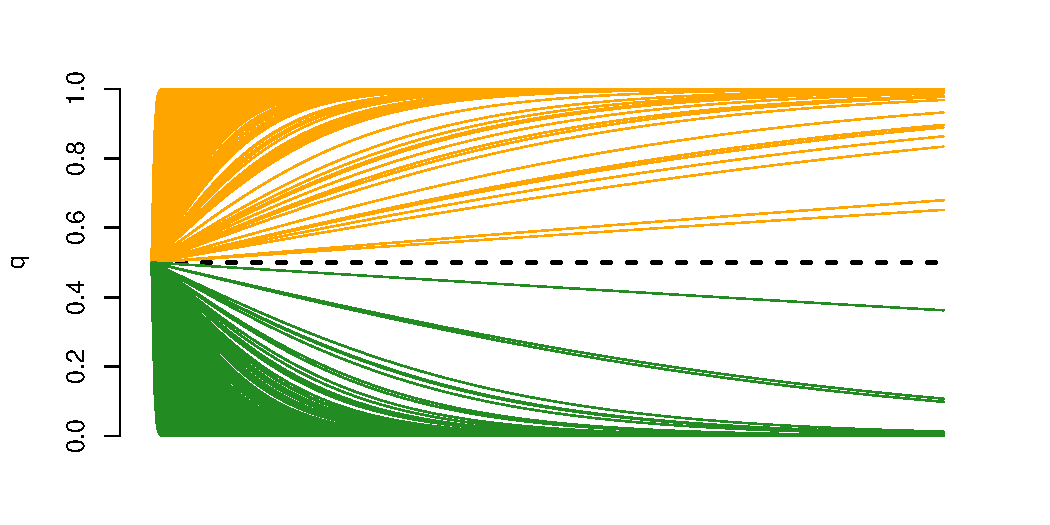
\includegraphics[width=\maxwidth]{figure/twocolumn-comp-1} 

}

\caption[Stuff]{Stuff}\label{fig:comp}
\end{figure}
\end{Schunk}
\begin{enumerate}
  \item[A] $\mu, \sigma$ and $N$ denote the mutation rate, the selection
    rate for a given allele, and the population size.
  \item[B] Under selective pressure, the allele is bound to either fixate or to
    simply die out. Whichever effect happens depends on the sign of $\sigma$,
    i.e.\ for $\sigma > 0$, the allele will eventually fixate with $q^1_i = 1$.
    In the contrasting case, the other allele will do the same. We can see this
    in \cref{fig:comp}, where we have separated randomly drawn positive values of $\sigma$ above     in orange, and correspondingly all negative values in green.
  \item[C] With no selective pressure, and mutations frequently producing either allele, as well as under no genetic drift, we will get the effect outlined in \cref{fig:stochc}, namely that the population will trend towards an equilibrium with an even split between the fractions. How fast this effect happens depends inherently on the mutation rate, which is signified in the figure by colour.  
\end{enumerate}
\begin{Schunk}
\begin{figure}[H]

{\centering 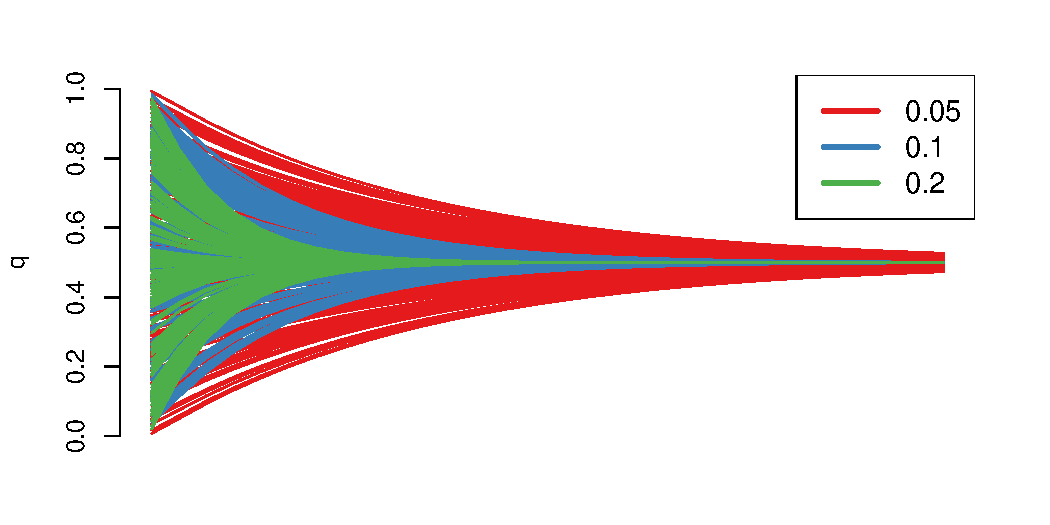
\includegraphics[width=\maxwidth]{figure/twocolumn-stochc-1} 

}

\caption[Stuff]{Stuff}\label{fig:stochc}
\end{figure}
\end{Schunk}
\begin{enumerate}
  \item[D] \Cref{fig:stochd} shows 500 drift-driven simulations initialised at $q = 0.2$. As we can see, the population on the large spreads out uniformly due to no pressure in going towards either end. We can argue about how likely it is on the grand scale that a single simulation will reach an allele fraction of $q = 1$ by considering Kimura's equation first. Since the overall expression reduces to $\dfrac{\partial p}{\partial t} = 0$ for $x = 1$, the probability for all initial conditions is some constant, which must depend on the initial condition combinatorically, as there are a different number of options to go in either direction from the beginning. The variance will only affect the rate at which we reach a certain point, so we can disregard this from our 
\end{enumerate}
\begin{Schunk}
\begin{figure}[H]

{\centering 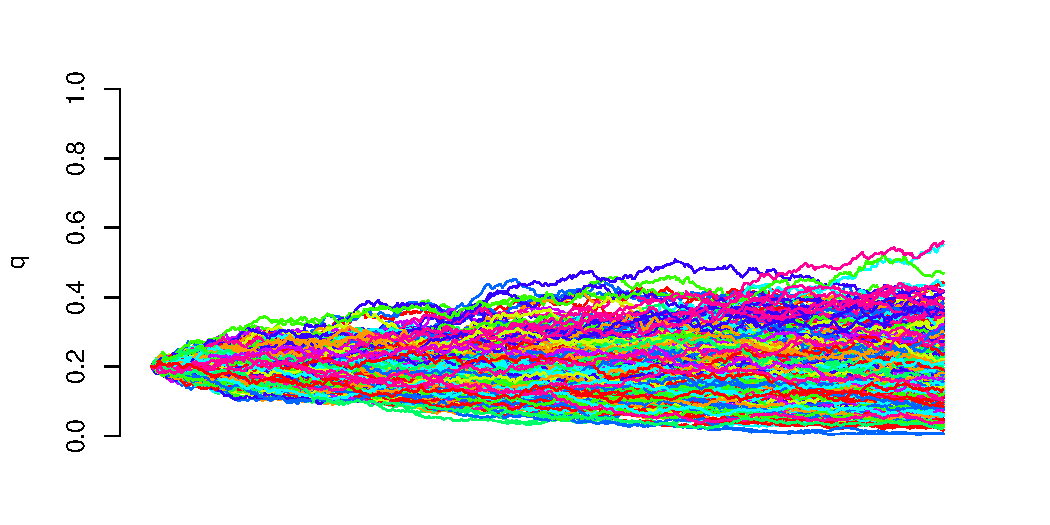
\includegraphics[width=\maxwidth]{figure/twocolumn-stochd-1} 

}

\caption[Stuff]{Stuff}\label{fig:stochd}
\end{figure}
\end{Schunk}

\subsection*{4 -- Time-dependent selection}
\begin{enumerate}
  \item[A] We separate our expression into two parts, and use induction to reason our way to the final answer. In particular, we have 
  
  \begin{align*}
  x(t')   =&~\dfrac{x_0e^{\sigma_1t'}}{1 - x_0 + x_0 e^{\sigma_1t'}} \\
  x(t>t') =&~\dfrac{x_{t'}e^{\sigma_2t}}{1  x_{t'} + x_{t'}e^{\sigma_2t}} = \\
          =&~\dfrac{x_0 e^{\sigma_2t + \sigma_1t'}}{\left(1 - x_0 + x_0e^{\sigma_1t'}\right)} \times \\
         &\times \dfrac{1}{\left(1 - \dfrac{x_0e^{\sigma_1t'} + x_0e^{\sigma_1t' + \sigma_2t}}{
            1 - x_0 + x_0e^{\sigma_1t'}}\right)} = \\
          =&~\dfrac{x_0e^{\sigma_1t' + \sigma_2t}}{1 - x_0 + x_0e^{\sigma_1t' + \sigma_2t}}
  \end{align*}
  for some arbitrary intervals where our $\sigma$'s are separable. Since we can repeat this process for any number of intervals, our corresponding exponent will equal a sum over the $\sigma-t$ products, which in the limit of our timesteps trending towards zero is equivalent to our sought-after integral.
  
\end{enumerate}

\begin{Schunk}
\begin{figure}[H]

{\centering 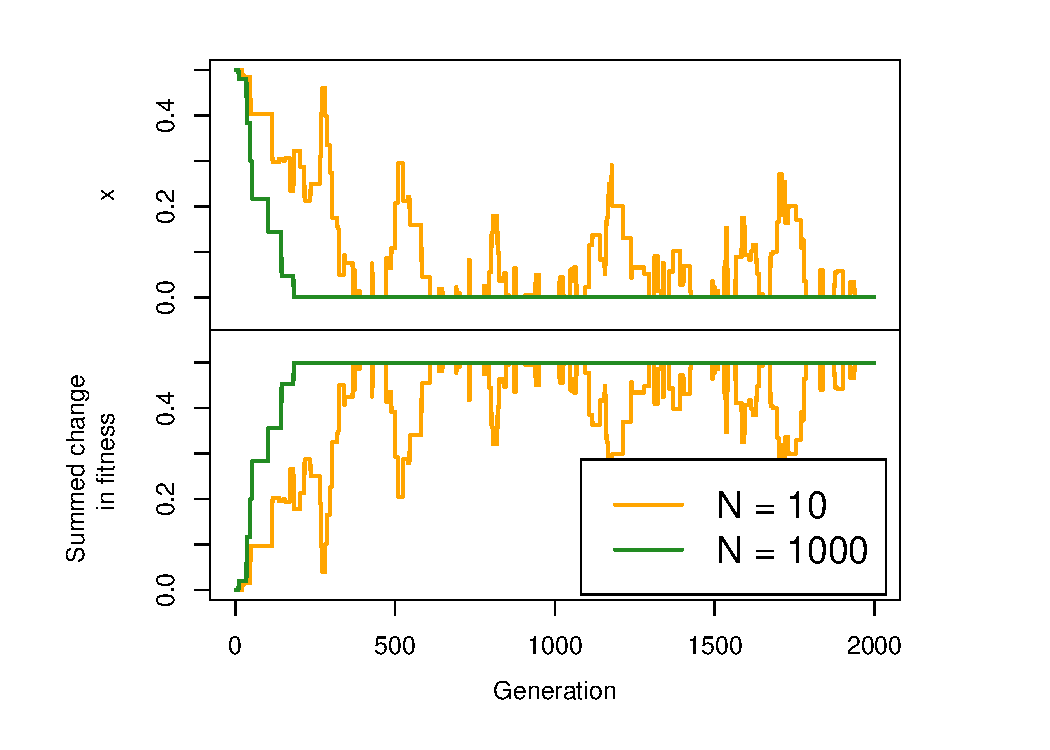
\includegraphics[width=\maxwidth]{figure/twocolumn-fisherb-1} 

}

\caption[Stuff]{Stuff}\label{fig:fisherb}
\end{figure}
\end{Schunk}
\begin{Schunk}
\begin{figure}[H]

{\centering 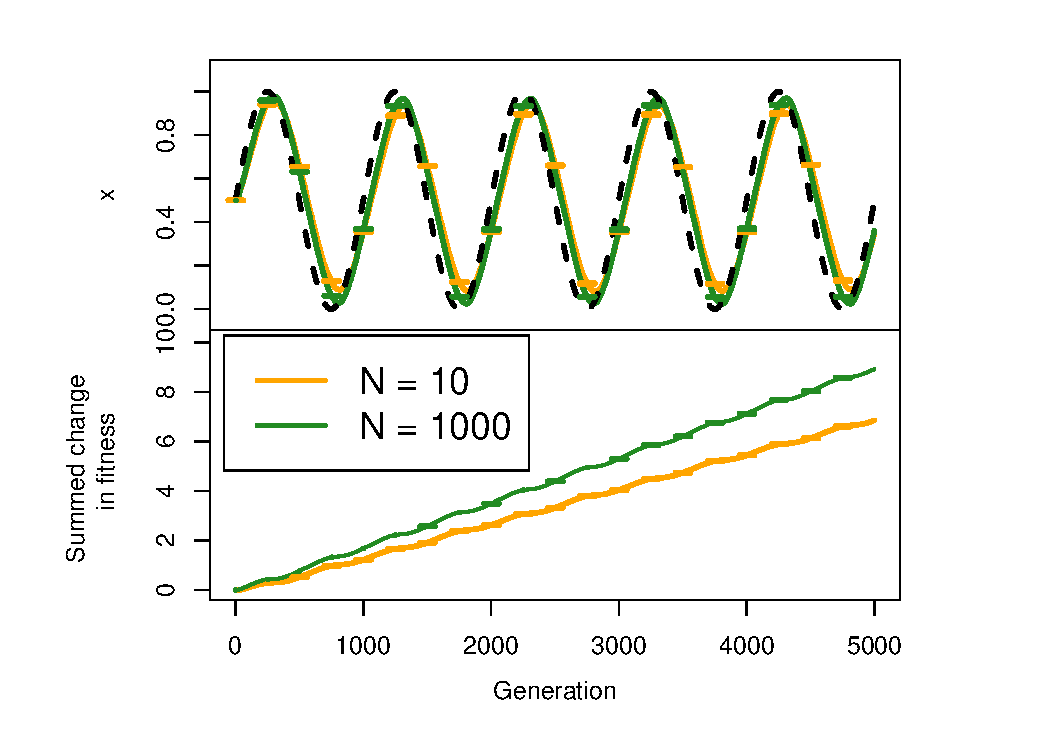
\includegraphics[width=\maxwidth]{figure/twocolumn-fisherc-1} 

}

\caption[Stuff]{Stuff}\label{fig:fisherc}
\end{figure}
\end{Schunk}

\begin{Schunk}
\begin{figure}[H]

{\centering 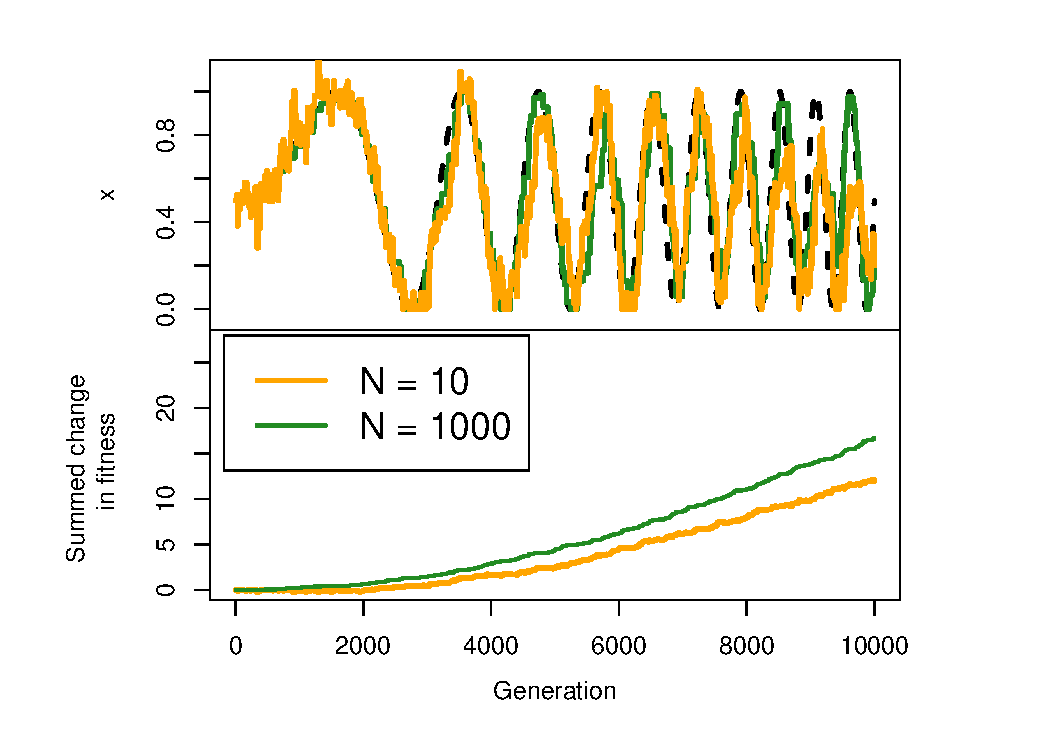
\includegraphics[width=\maxwidth]{figure/twocolumn-fisherd-1} 

}

\caption[Stuff]{Stuff}\label{fig:fisherd}
\end{figure}
\end{Schunk}
\begin{Schunk}
\begin{figure}[H]

{\centering 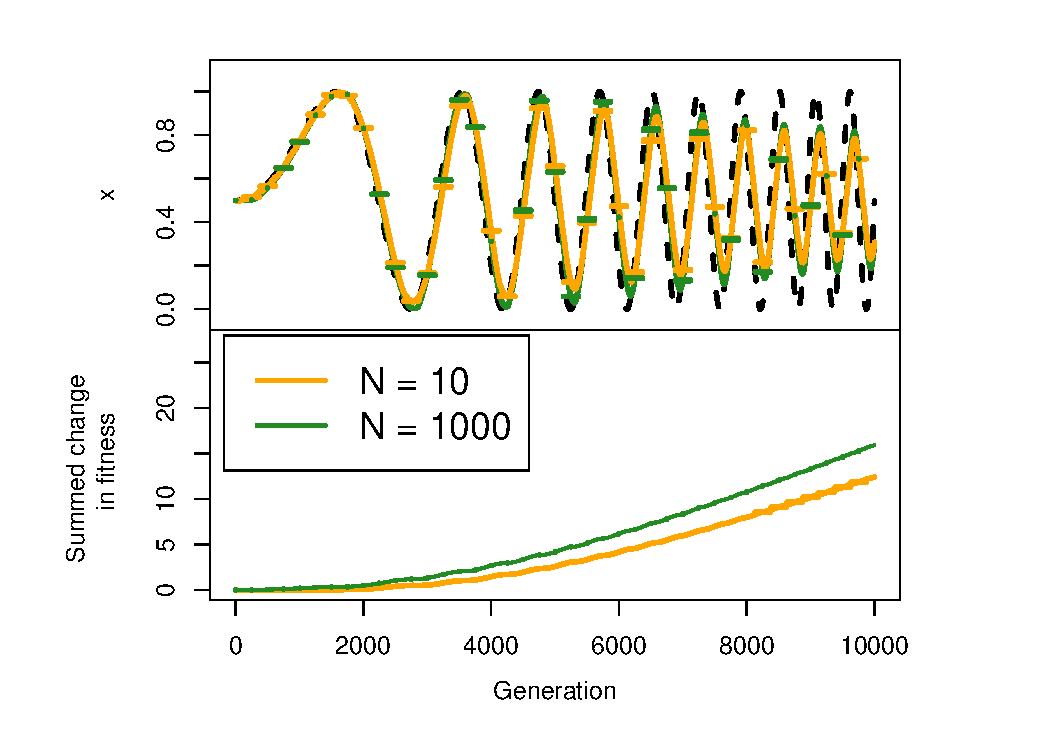
\includegraphics[width=\maxwidth]{figure/twocolumn-fisherd_ext-1} 

}

\caption[Stuff]{Stuff}\label{fig:fisherd_ext}
\end{figure}
\end{Schunk}

Biological systems: Some populations have a harder time adapting.

\bibliography{references}
\end{multicols*}



\end{document}
